\subsubsection{ProvDAL}
ProvDAL is a service the interface of which is organized around one main parameter, the \urlparam{\bf ID} of an entity (obs\_publisher\_did of an ObsDataSet for example), activity or an agent.
The response is given in one of the following formats: \urlparam{PROV-N}, \urlparam{PROV-JSON}, \urlparam{PROV-XML}, \urlparam{PROV-VOTABLE}.
Additional parameters can complete the \urlparam{ID} to refine the query: \urlparam{\bf FORMAT} allows to choose the output format. \urlparam{\bf DEPTH} gives the number of relations that shall be tracked along the provenance history, independent of the type of relation. Its value is either 0, a positive integer or \urlparam{ALL}. If this parameter is omitted, the default is \urlparam{ALL}, which returns the complete provenance history that the service has stored or the provenance according to a maximum depth number that the server allows.

The \urlparam{ID} parameter is allowed more than once in order to retrieve provenance details for several activities or datasets at the same time. Here are a few example requests:

\begin{verbatim}
{provdal-base-url}?ID=rave:dr4&FORMAT=PROV-JSON
{provdal-base-url}?ID=rave:dr4&ID=rave:act_irafReduction&DEPTH=2
\end{verbatim}

\noindent
The format can also be specified via the HTTP accept header, e.g.
\begin{verbatim}
wget -d --header="Accept: application/json" \
   {provdal-base-url}?ID=rave:dr4
\end{verbatim}
would return the provenance information in \urlparam{PROV-JSON} format.
\noindent
If both \urlparam{FORMAT} and the accept header are used and \urlparam{FORMAT} specifies a format that is incompatible with the HTTP accept header, then the service should return with a HTTP status 406: Not Acceptable.

For services which allow tracking the provenance information forward, e.g. in order to check for which activities an entity was used, the optional parameter \urlparam{\bf DIRECTION} can be set to \urlparam{FORTH}. Its default value is \urlparam{BACK}. This influences the direction in which the used, wasGeneratedBy, wasDerivedFrom and wasInfluencedBy relations are followed.

The provenance data model defines also the hierarchical relations \emph{hadMember} for entity collections and \emph{hadStep} for activityFlows. If a node belongs to a collection or activityFlow, these relations shall be returned as well, independent of the specified tracking direction.
If one is interested in more details and wants to follow the \emph{members} of an entity collection or the \emph{steps} of an activityFlow, these can be included by setting the optional parameter \urlparam{\bf MEMBERS} or \urlparam{\bf STEPS} to \urlparam{TRUE}, respectively. The default is \urlparam{FALSE}.

By default, it is recommended to stop any further tracking at an agent node, unless an additional optional parameter \urlparam{\bf AGENT} is set to \urlparam{TRUE}. Note that this means that the request for any agent will always return just the agent node itself and nothing else, unless \urlparam{AGENT=TRUE} is used. Thus, if one wants to know which entities and activities an agent has influenced, the request looks like this:

\begin{verbatim}
{provdal-base-url}?ID=org:rave&AGENT=TRUE&DEPTH=1
\end{verbatim}

\noindent
\urlparam{DEPTH=1} was used here in order to avoid following the found entities and activities any further.

%\comment{Maybe it's better to use DEPTH and DIRECTION instead of FORWARD and BACKWARD. Reason: if a service just implements the backward direction, then it's weird to call something ``backward'' if there is no ``forward'' as well. DEPTH is also a commonly used word when refering to graphs and numbers of relations.}


\begin{figure}[h]
\centering
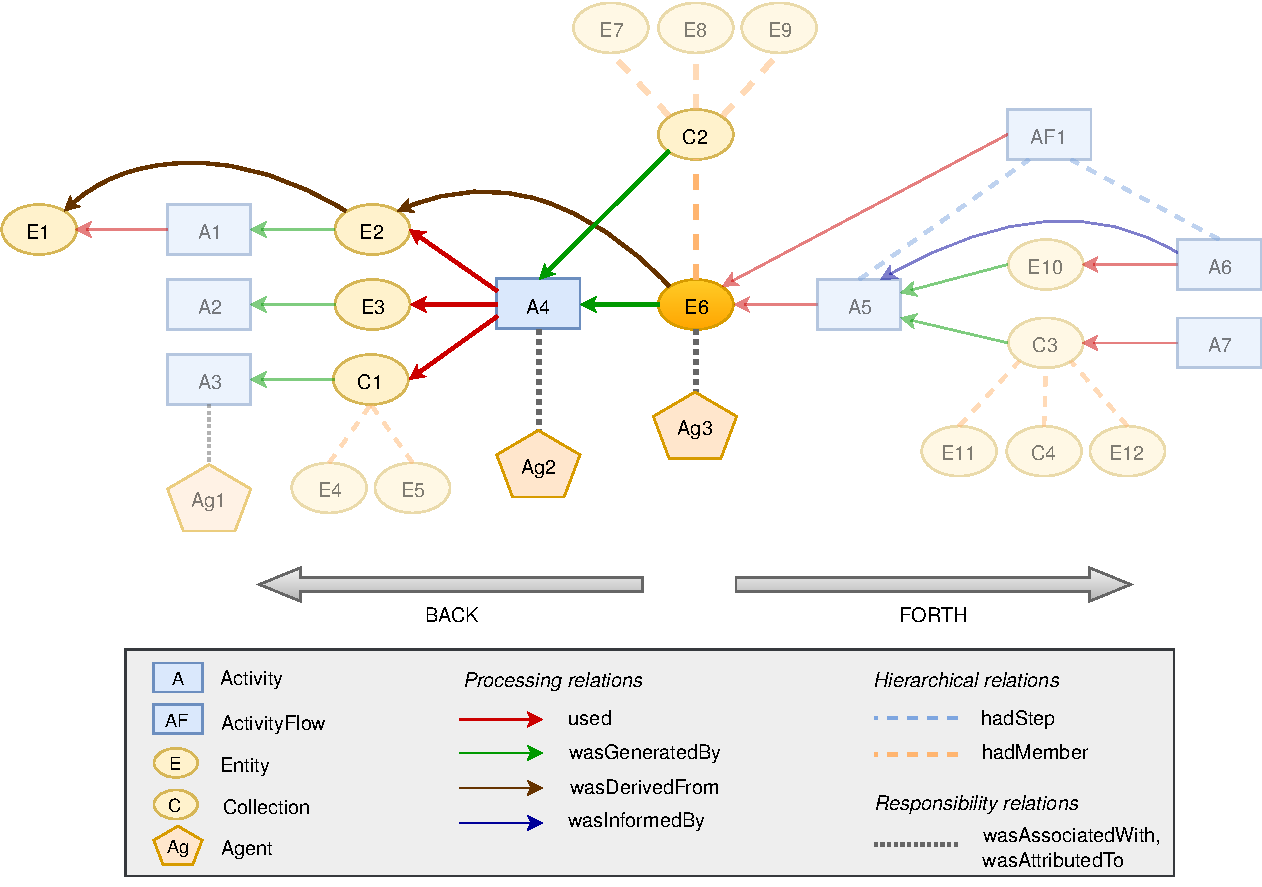
\includegraphics[width=1.0\textwidth]{provenance-graph-example-depth2.pdf}
\caption{An example provenance graph, highlighting the objects and relations returned from a ProvDAL service with ID=E6 and \urlparam{DEPTH}=2. The \urlparam{BACK} and \urlparam{FORTH} values for \urlparam{DIRECTION} are only important for the processing relations (solid lines). Hierarchial (dashed) and responsibility relations (dotted) are only followed ``upwards'' and towards agents by default. If they should also be followed in the other direction, then the additional optional parameters \urlparam{MEMBERS}, \urlparam{STEPS} and \urlparam{AGENT} need to be set to \urlparam{TRUE}.}
\label{fig:provenance-graph-example}
\end{figure}


A ProvDAL service MUST implement the parameters \urlparam{ID}, \urlparam{DEPTH} and \urlparam{FORMAT}; the remaining parameters are optional.
If a service does not implement the optional parameters, but they appear in the request, then the service should return with an error.

Table~\ref{tab:provdal-parameters} summarizes the parameters for such a ProvDAL service interface.

\begin{table}[h]
\small
\begin{tabulary}{1.0\textwidth}{@{}p{0.17\textwidth}p{0.22\textwidth}p{0.53\textwidth}@{}}
%{llp{0.2\textwidth}p{0.3\textwidth}}
\toprule
\head{Parameter} & \head{Value/options} & \head{Description}\\\hline
\midrule
\textbf{\urlparam{ID}} & qualified \urlparam{ID} & a valid qualified identifier for an entity or activity (can occur multiple times)\\
\textbf{\urlparam{DEPTH}} & 0,1,2,..., \urlparam{\underline{ALL}} &  number of relations to be followed or \texttt{ALL} for everything, independent of the relation type\\
\textbf{\urlparam{FORMAT}} & \urlparam{PROV-N}, \newline\urlparam{PROV-JSON}, \newline\urlparam{PROV-XML}, \newline\urlparam{PROV-VOTABLE} & serialisation format of the response\\\hline
\urlparam{DIRECTION} & \urlparam{\underline{BACK}}, \urlparam{FORTH} & \urlparam{BACK} = track the provenance history, \newline\urlparam{FORTH} = explore the results of activities and where entities have been used\\
\urlparam{MEMBERS} & \urlparam{TRUE} or \urlparam{\underline{FALSE}} & if \urlparam{TRUE}, retrieve and track members of collections\\
\urlparam{STEPS} & \urlparam{TRUE} or \urlparam{\underline{FALSE}} & if \urlparam{TRUE}, retrieve and track steps of activityFlows\\
\urlparam{AGENT} & \urlparam{TRUE} or \urlparam{\underline{FALSE}} & if \urlparam{TRUE}, retrieve all relations for agents, i.e. find out what an agent is responsible for\\
\bottomrule
\end{tabulary}
\caption{ProvDAL request parameters. Options that are \textbf{required} to be implemented by ProvDAL services are marked with bold face. \underline{Default} values are underlined.}
\label{tab:provdal-parameters}
\end{table}


